\documentclass{beamer}
\usetheme{CambridgeUS}
\usepackage[utf8]{inputenc}
\usepackage{amsmath}
\usepackage[spanish]{babel}
\usepackage{graphicx}

\title
{Detección de cúmulos de galaxias}
\subtitle{Corrimiento al rojo fotométrico}
\author[Vargas, Márquez]
{Ignacio Vargas Cordero \and Carlos Oscar Márquez Rangel}
\institute[]
{
	\inst{}
	Facultad de Ciencias\\
	UNAM
}
\date[26/02/18]
{\today}
\subject{Laboratorio de Física Contemporánea}

\begin{document}
	
	\frame{\titlepage}
	
	\begin{frame}
		\frametitle{Objetivos}
		Los objetivos de la práctica fueron los siguientes:
		\begin{itemize}
			\item Entender los conceptos de corrimiento al rojo y su relación con la expansión del universo; las distancias en cosmología; flujo y luminosidad; y encontrar el mejor modelo cosmológico mediante un ajuste de $\chi^2$.
			\item Todo lo anterior para obtener el mejor corrimiento al rojo fotométrico para galaxias rojas reales, verificando los resultados con la información espectroscópica disponible.
		\end{itemize}
    \end{frame}

\begin{frame}
\frametitle{Conceptos básicos}
Los conceptos utilizados a lo largo de toda la práctica fueron los siguientes:
\begin{itemize}
	\item Corrimiento al rojo: Este ocurre cuando incrementa la longitud de onda de la radiación electromagnética de un objeto, lo que provoca un corrimiento al extremo tojo del espectro. Dado que el Universo se encuentra en expansión, las galaxias lejanas presentan un corrimiento $z$ que es el que utilizamos a lo largo de la práctica.
	\item Corrimiento al rojo fotométrico: Es una estimación de la velocidad de recesión de un objeto astronómico sin tener que medir su espectro. Esta técnica utiliza fotometría (esto es, el brillo del objeto a través de distintos filtros/bandas) para determinar $z$.
\end{itemize}
También se utilizó un \textbf{corte}, el cual nos sirvió para separar galaxias rojas de estrellas. En esta práctica se utilizó un corte de $r_{psf} - r_{model} > 0.3$.
\end{frame}

	\begin{frame}
\frametitle{Ecuaciones en cosmología}
Empezamos definiendo el factor de escala del universo por $a$, el cual tiene un valor de $1$ hoy. Con esto definimos la ecuación de Hubble
$$H^2(a)=\bigg(\frac{\dot{a}}{a}\bigg)^2$$

Considerando un universo plano y el corrimiento al rojo $z$, la función de Hubble estará dada por
%\begin{equation*}
$$H(z)=H_0\sqrt{\Omega_M(1+z)^3+\Omega_R(1+z)^4+\Omega_\Lambda}$$
%\end{equation*}


\end{frame}

	\begin{frame}
		\frametitle{Distancias en cosmología}
		Existen varias definiciones para la distancia. La principal utilizada a lo largo de la práctica fue la distancia de Comoving
		$$\chi(z_{emmit})=\frac{c}{H_0}\int_{0}^{z_{emmit}} \frac{dz}{H_0\sqrt{\Omega_M(1+z)^3+\Omega_R(1+z)^4+\Omega_\Lambda}}$$
		Otras incluyen la distancia de luminosidad 
		$$D_l(z_{emmit})=\frac{c(1+z_{emmit})}{H_0}\int_{0}^{z_{emmit}} \frac{dz}{H_0\sqrt{\Omega_M(1+z)^3+\Omega_R(1+z)^4+\Omega_\Lambda}}$$
		Y la distancia angular
		$$D_A(z_{emmit})=\frac{c}{H_0(1+z_{emmit})}\int_{0}^{z_{emmit}} \frac{dz}{H_0\sqrt{\Omega_M(1+z)^3+\Omega_R(1+z)^4+\Omega_\Lambda}}$$
	\end{frame}

\begin{frame}
\frametitle{Ecuaciones para observaciones astronómicas}
Definimos el flujo como la energía de los fotones que recibe una área de $1 cm$ en $1 s$. La relación entre el flujo y la luminosidad, a una longitud de onda $\lambda$ dada, es
	$$f(\lambda)=\frac{L(\lambda)}{4\pi d^2}$$
Tomando en cuenta los efectos del corrimiento al rojo tenemos
	$$f(\lambda)=\frac{L(\lambda /(1+z))}{4\pi D^2_L(z)}$$
Con 
$$D^2_L(z)=(1/z)\chi (z)$$

\end{frame}

\begin{frame}
\frametitle{Magnitud y color en astronomía}
La magnitud de un objeto se refiere a la medición logarítmica de su brillo en una banda bien definida. Existe la magnitud abosoluta y la magnitud aparante, esta última siendo el brillo de un objeto tal y como aparece en el cielo nocturno visto desde la Tierra. La magnitud aparente está dada por:
$$mag_b=-2.5 \log_{10} \bigg(\frac{f^{mes}_b}{f^{ref}_b}\bigg)$$
Sin embargo, lo que nos interesa es la diferencia entre magnitudes:
$$mag_{b1}-mag_{b2}=-2.5\bigg[\log_{10} \bigg(\frac{f^{mes}_{b1}(1M_\odot)f^{ref}_{b2}}{f^{mes}_{b2}(1M_\odot)f^{ref}_{b1}}\bigg)\bigg]$$
$$=mag_{b1}(1M_\odot)-mag_{b2}(1M_\odot)$$
A la diferencia entre magnitudes aparentes la llamamos \textbf{color}.
%M_\odot
\end{frame}

\begin{frame}
\frametitle{SDSS}
La Sloan Digital Sky Survey (SDSS) ha mapeado cerca de un tercio del cielo nocturno en 5 bandas (u, g, r, i y z). Lo que se obtiene es un catálogo para casi 500 mil millones de objetos únicos. En particular utilizaremos la Extended Baryon Oscillation Spectroscopic Survey (eBOSS). Con esta base de datos haremos nuestros programas.

\begin{columns}
	\begin{column}{6cm}
		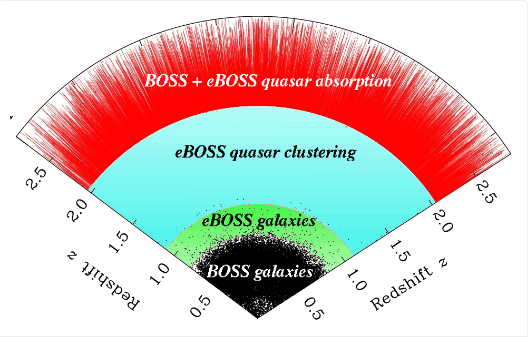
\includegraphics[width=\columnwidth]{eBoss.png} 
	\end{column}
\end{columns}

\end{frame}

%\begin{frame}
%\frametitle{Densidad de energía espectral (SED)}
%
%\end{frame}

\begin{frame}
\frametitle{Corrimiento al rojo fotométrico (Foto-z)}

\begin{itemize}
	\item Usando este simple modelo, tenemos una herramienta útil para determinar el corrimiento al rojo fotométrico. Ahora debemos explorar el concepto de Foto-z: El espectro de una galaxia roja presenta un quiebre en 4000Å en el marco de referencia en reposo de la galaxia. Este quiebre crea una diferencia en la magnitud de las bandas el cual depende fuertemente del corrimiento al rojo observado. Más aún, podemos determinar el corrimiento al rojo que modele el color mejor observado.
	\item Se utilizarán los datos disponibles para crear un algoritmo que determine el Foto-z para galaxias SDSS.
\end{itemize}


%Using this simple model, you will see that you have a nice tool to determine the photometric redshift. But whatis a photo-z? As you can see on the figure 3, the spectrum of a red galaxy present a break at4000Å in the galaxyrestframe. This break creates a difference in the magnitude of the bands which strongly depends on the redshiftof observation. Using the colors, so the difference between magnitudes, we can determine which redshift allowsto model the best the observed color.
\end{frame}

\begin{frame}
\frametitle{Descripción de los programas y resultados}
Nuestros programas se dividen en dos grupos:
\begin{itemize}
	\item Variando el valor del corrimiento al rojo $z$, obtenemos curvas para la función de Hubble, así como para las distancias (medidas en parsecs) de Comoving, luminosidad y angular.
	\item Obtenemos los valores de las bandas y de $z$ en un cierto punto del cielo, con un radio de 40 arcominutos, para obtener y graficar los colores dependientes de $z$, así como discriminar las cúmulos de galaxias de estrellas solas y finalmente realizar un ajuste de $\chi^2$, verificando que el modelo es bueno como una primera aproximación.
\end{itemize}

Para hacer estos programas y el ajusto utilizamos un modelo de corrimiento al rojo ideal, el cual comparamos con los datos reales obtenidos de eBOSS.

\end{frame}


\begin{frame}
\frametitle{Función de Hubble dependiente de z}
\begin{columns}
	\begin{column}{10cm}
		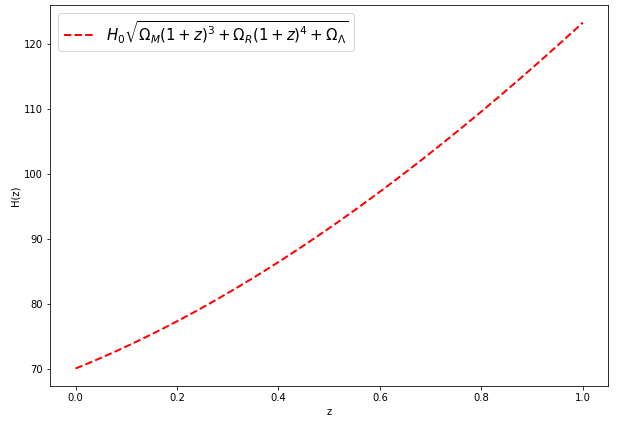
\includegraphics[width=\columnwidth]{8.png} 
\end{column}
\end{columns}
\end{frame}


\begin{frame}
    \frametitle{Distancias cosmológicas} 
\begin{columns}
	\begin{column}{10cm}
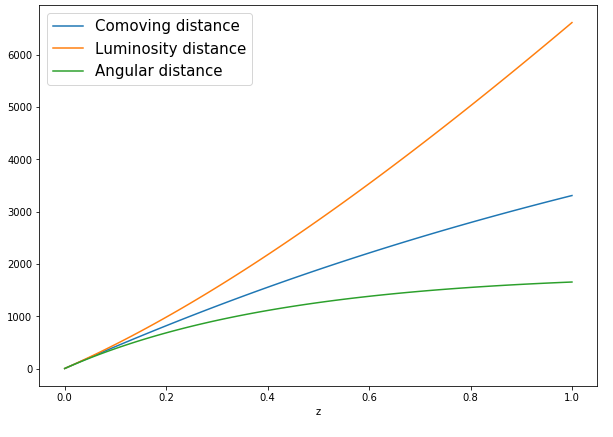
\includegraphics[width=\columnwidth]{discosm0.png} 
\end{column}
\end{columns}
\end{frame}

\begin{frame}
\frametitle{g-u}
\begin{columns}
	\begin{column}{10cm}
		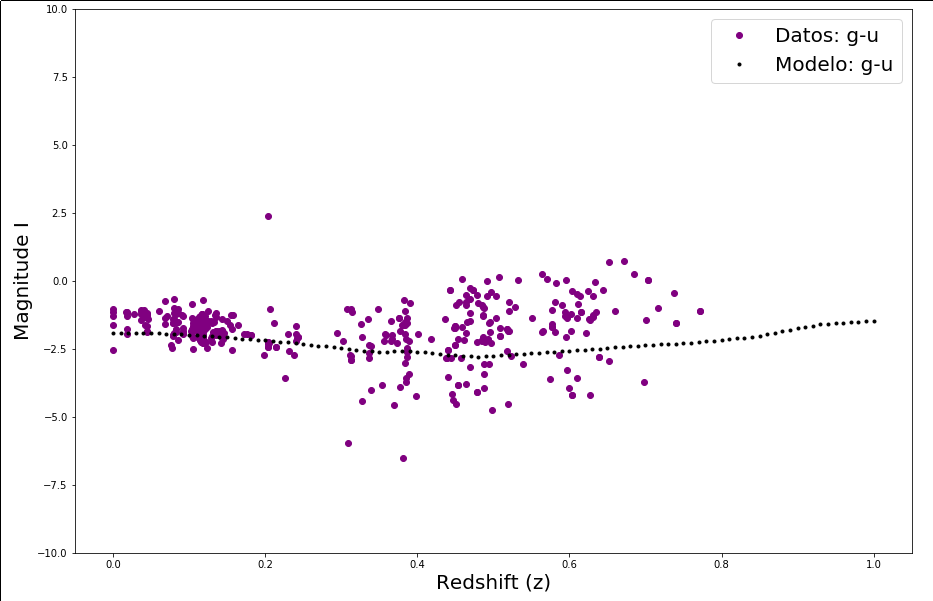
\includegraphics[width=\columnwidth]{gu.png} 
	\end{column}
\end{columns}
\end{frame}

\begin{frame}
\frametitle{g-r}
\begin{columns}
	\begin{column}{10cm}
		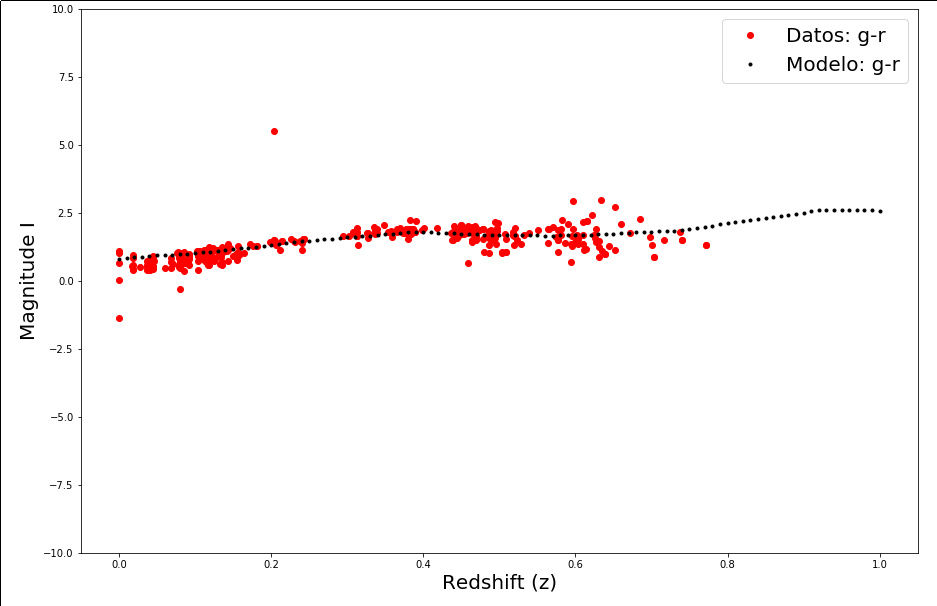
\includegraphics[width=\columnwidth]{gr} 
	\end{column}
\end{columns}
\end{frame}

\begin{frame}
\frametitle{g-i}
\begin{columns}
	\begin{column}{10cm}
		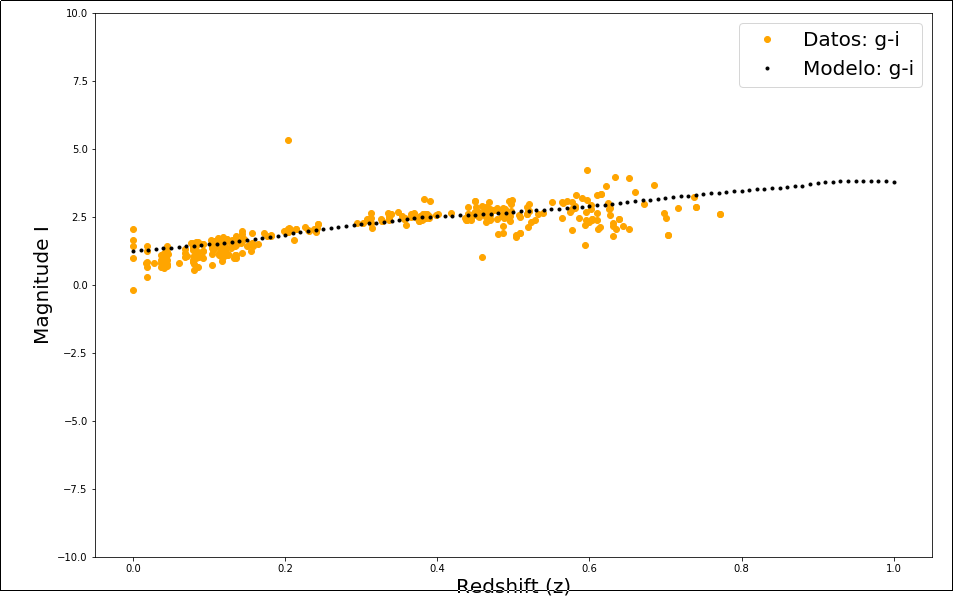
\includegraphics[width=\columnwidth]{gi.png} 
	\end{column}
\end{columns}
\end{frame}

\begin{frame}
\frametitle{g-z}
\begin{columns}
	\begin{column}{10cm}
		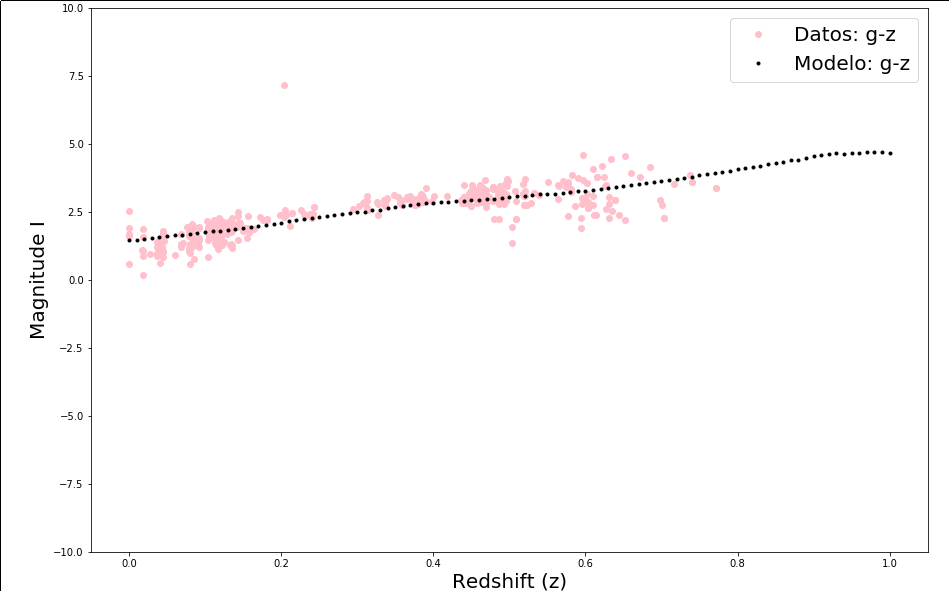
\includegraphics[width=\columnwidth]{gz.png} 
	\end{column}
\end{columns}
\end{frame}

\begin{frame}
\frametitle{Corte}
\begin{columns}
	\begin{column}{10cm}
		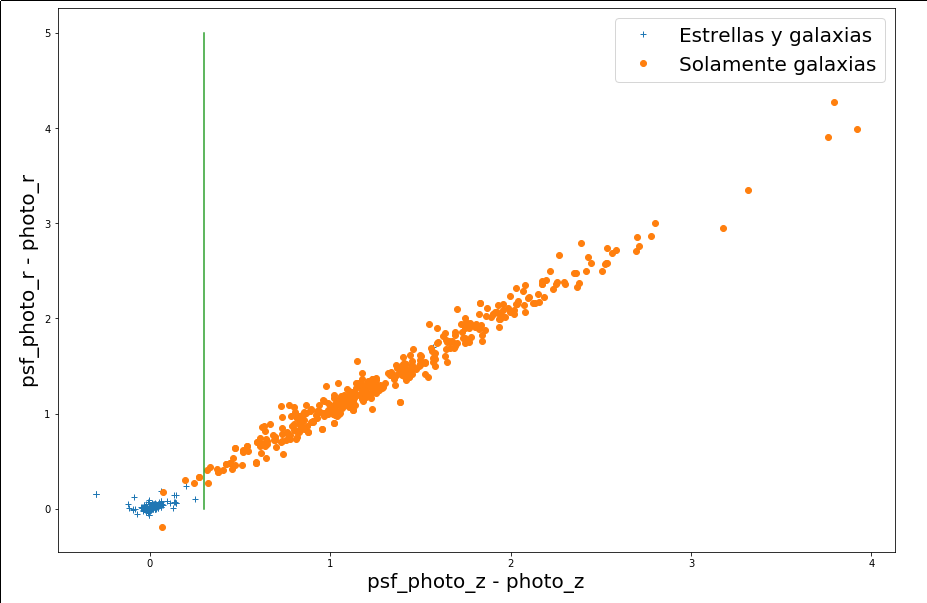
\includegraphics[width=\columnwidth]{corte.png} 
	\end{column}
\end{columns}
\end{frame}

\begin{frame}
\frametitle{Ejemplo de $\chi^2$}
\begin{columns}
	\begin{column}{10cm}
		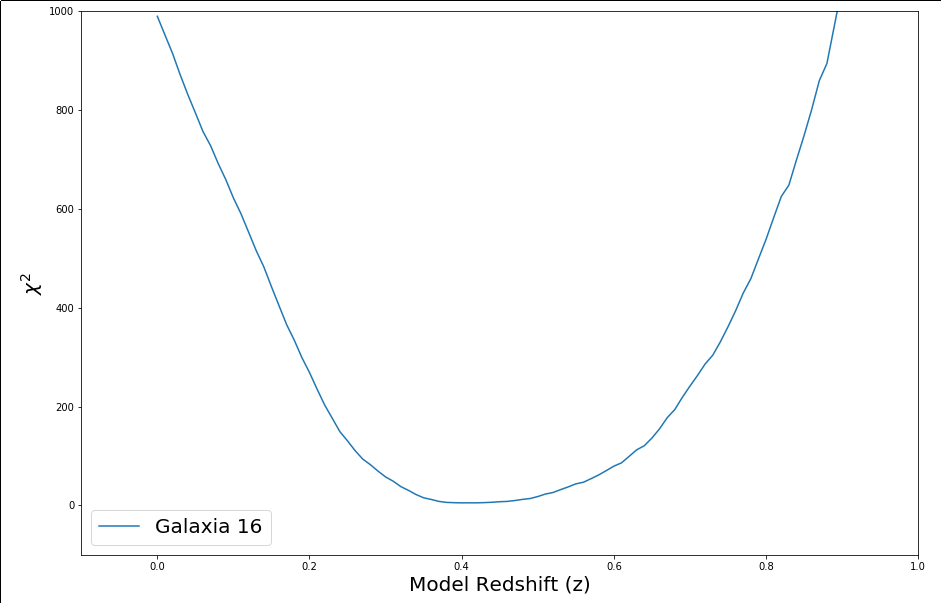
\includegraphics[width=\columnwidth]{chi2.png} 
	\end{column}
\end{columns}
\end{frame}

\begin{frame}
    \frametitle{Photometric vs Spectroscopic Redshift}
\begin{columns}
	\begin{column}{10cm}
		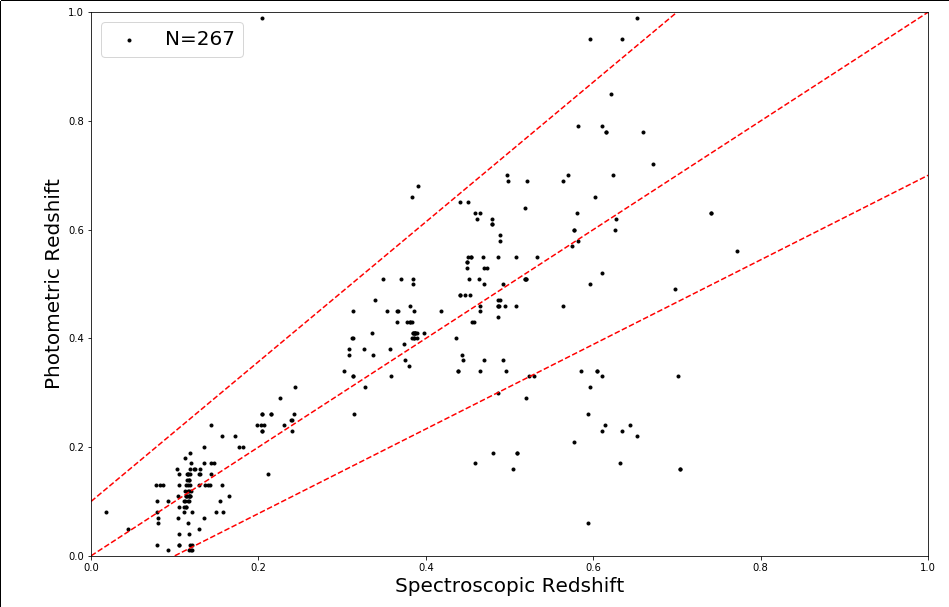
\includegraphics[width=\columnwidth]{vs.png} 
	\end{column}
\end{columns}
\end{frame}

\begin{frame}
    \frametitle{Photometric - Spectroscopic Redshift}
\begin{columns}
	\begin{column}{10cm}
		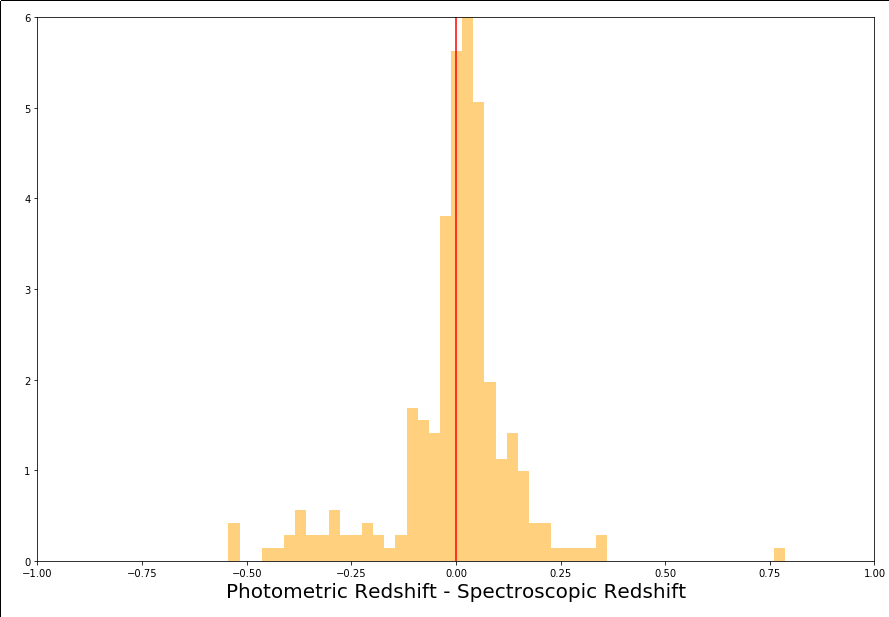
\includegraphics[width=\columnwidth]{hist.png} 
	\end{column}
\end{columns}
\end{frame}

\begin{frame}
\frametitle{Conclusiones}

\begin{itemize}
	\item Obtuvimos las gráficas para la función de Hubble y las distancias, viendo como evoluciona el comportamiento con respecto al corrimiento $z$.
	\item Calculamos los colores y pudimos hacer los cortes para discernir entre galaxias rojas y estrellas.
	\item Realizamos el ajuste en $\chi^2$ para las galaxias rojas tomando en cuenta los 4 colores.
	\item Con el ajuste de $\chi^2$ vimos que el modelo es muy bueno como primera aproximación. 
\end{itemize}

\end{frame}

\end{document}
